% Exercise Template
% A LaTeX template for typesetting exercise in Persian (with cover page).
% By: Reza Adinepour
% Github: github.com/rezaAdinepour

\documentclass[12pt]{exam}

\usepackage{setspace}
\usepackage{listings}
\usepackage{graphicx,wrapfig}
\usepackage{caption}
\usepackage{subcaption}
\usepackage{multirow}
\usepackage{matlab-prettifier}
\usepackage{amsmath}
\usepackage{multicol}
\usepackage[hidelinks]{hyperref}



\usepackage[utf8]{inputenc}
\usepackage{fourier} 
\usepackage{array}
\usepackage{makecell}

\renewcommand\theadalign{bc}
\renewcommand\theadfont{\normalsize}
\renewcommand\theadgape{\Gape[4pt]}
\renewcommand\cellgape{\Gape[4pt]}


\usepackage[margin=25mm]{geometry}
\usepackage{xepersian}
\settextfont{XB Niloofar}

\newcommand{\class}{\ThesisClass}

\singlespacing
\parindent 0ex

\begin{document}


% -------------------------------------------------------
%  Thesis Information
% -------------------------------------------------------

\newcommand{\ThesisType}
{سمینار}  % پایان‌نامه / رساله
\newcommand{\ThesisDegree}
{کارشناسی ارشد گرایش معماری کامپیوتر}  % کارشناسی / کارشناسی ارشد / دکتری
\newcommand{\ThesisMajor}
{مهندسی کامپیوتر}  % مهندسی کامپیوتر
\newcommand{\ThesisTitle}
{تمرین شبیه‌سازی سری ۳}
\newcommand{\ThesisAuthor}
{\href{https://github.com/rezaAdinepour/M.Sc-AUT/tree/main/Advanced Computer Architecture}{\textcolor{black}{رضا آدینه پور}} - ۴۰۲۱۳۱۰۵۵}
\newcommand{\ThesisSupervisor}
{جناب آقای دکتر فربه}
\newcommand{\ThesisDate}
{۲۳ آذر ۱۴۰۲}
\newcommand{\ThesisDepartment}
{دانشکده مهندسی کامپیوتر}
%\newcommand{\ThesisUniversity}
%{دانشگاه صنعتی امیرکبیر}

% -------------------------------------------------------
%  English Information
% -------------------------------------------------------

%\newcommand{\EnglishThesisTitle}{A Standard Template for Course Exercise}


\pagestyle{empty}

\begin{center}


\includegraphics[scale=0.15]{images/aut-fa.png}

%\vspace{0.5cm}
%\ThesisUniversity \\[-0.3em]
%\vspace{0.5cm}
\large\ThesisDepartment

\begin{large}
\vspace{0.5cm}


%\ThesisMajor

\end{large}

\vspace{1.5cm}

{عنوان:}\\[1.2em]
{\LARGE\textbf{\ThesisTitle}}\\ 
\vspace{1cm}
% \begin{latin}
% {\Large\textbf\EnglishThesisTitle}
% \end{latin}

\vspace{2cm}

{نگارش}\\[.5em]
{\large\textbf{\ThesisAuthor}}

\vspace{1.5cm}

{استاد مربوطه}\\[.5em]
{\large\textbf{\ThesisSupervisor}}

\vspace{1cm}



\vspace{2cm}

\ThesisDate

\end{center}

\newpage


% These commands set up the running header on the top of the exam pages
\pagestyle{head}
\firstpageheader{}{}{}
\runningheader{صفحه \thepage\ از \numpages}{}{\class}
\runningheadrule

\vspace{0pt}


\begin{questions}
	\pointpoints{نمره}{نمره}
	
	\section*{سوالات تئوری}
	\question
\textbf{به سوالات زیر پاسخ دهید:‌ }

\begin{enumerate}
	\item 
	\lr{PUM} چیست و کدام نوع حافظه‌ها برای آن بیشتر استفاده می‌شوند؟ توضیح دهید چرا هر نوع حافظه استفاده می‌شود.
	
	\textbf{پاسخ: }
پردازش در حافظه (\lr{PUM}) یک کانسپت محاسباتی است که در آن برخی از محاسبات ساده مانند جمع و ضرب به جای انتقال داده‌ها بین \lr{CPU} و حافظه، مستقیما در حافظه انجام می‌شوند.

معمولا از \lr{DRAM}، \lr{SRAM} و \lr{NVM} ها در \lr{PUM} استفاده می‌شود. که در ادامه به بررسی مزایا و معایب استفاده از هرکدام می‌پردازیم.

\lr{DRAM} ها
به دلیل اینکه رایج‌ترین نوع حافظه فرار با تراکم بالا و هزینه کم به ازای هر بیت هستند، به طور گسترده استفاده می‌شود. ویژگی‌های خازنی سلول‌های \lr{DRAM} امکان انجام تکنیک‌های محاسباتی درون حافظه مانند عملیات منطقی و حسابی را فراهم می‌کند.

مزایا: تراکم بالا، ارزان است.\\
معایب: فرار، نیاز به تازه‌سازی دوره‌ای و معمولاً تأخیر بیشتر نسبت به \lr{SRAM}.

اما در مقابل  \lr{SRAM} زمان‌های تأخیر کمتری و زمان دسترسی سریعتری نسبت به \lr{DRAM} دارد و در مواردی که سرعت برای ما بسیار مهم است، (مانند \lr{Cache})، استفاده می‌شود. توانایی حفظ حالت بدون نیاز به تازه‌سازی، آن را برای عملیات‌های \lr{PUM} مناسب می‌سازد.

مزایا: زمان‌های دسترسی سریع نسبت به \lr{DRAM}، عدم نیاز به تازه‌سازی.\\
معایب: تراکم کمتر و هزینه بیشتر به ازای هر بیت نسبت به \lr{DRAM}.


درمقابل حافظه‌های فرار، انواع حافظه‌های غیر فرار مانند \lr{Flash}، \lr{PCM} و \lr{ReRAM} به دلیل نگه داشتن داده بدون برق، برای ذخیره‌سازی پایدار و محاسبات مناسب هستند. این حافظه‌ها می‌توانند برخی عملیات منطقی را درون سلول‌های حافظه انجام دهند.

مزایا: غیر فرار بودن. \\
معایب: عموماً سرعت نوشتن کندتر و دوام کمتر نسبت به \lr{DRAM} و \lr{SRAM}.
	
	
	
	
	
	\item 
	نقاط ضعف \lr{UPMEM} چیست؟
	
	\textbf{پاسخ:} از نقاط ضعف \lr{UPMEM} ها می‌توان به موارد زیر اشاره کرد:
	
	
	\begin{enumerate}
		\item انعطاف‌پذیری و قابلیت برنامه‌ریزی محدود:\\
معماری \lr{PIM UPMEM} برای انواع خاصی از عملیات (مانند وظایف داده‌محور مانند جست‌وجو در پایگاه داده و تحلیل) است. ممکن است به اندازه CPU یا GPUهای سنتی عمومی و همه‌منظوره نباشد، که کاربرد آن را به بارهای کاری خاص محدود می‌کند.
		
		
		
		\item یکپارچه‌سازی و سازگاری:\\
یکپارچه‌سازی ماژول‌های \lr{PIM UPMEM} با سیستم‌های موجود می‌تواند چالش‌برانگیز باشد. ممکن است مشکلات سازگاری با معماری‌های حافظه و پردازنده فعلی به وجود بیاید که نیاز به اصلاحات در کانفیگ نرم‌افزار و سخت‌افزار دارد.
		
		
		
		\item مسائل مربوط به کارایی انرژی:\\
در حالی که \lr{PIM} هدفش کاهش مصرف انرژی با حداقل‌کردن حرکت داده‌ها بین حافظه و \lr{CPU} است،‌ صرفه‌جویی واقعی در انرژی می‌تواند وابسته به بار کاری باشد. برخی عملیات ممکن است همچنان مصرف انرژی قابل توجهی داشته باشند، به خصوص اگر منطق \lr{PIM} به‌طور کامل برای آن کاربرد به‌خصوص بهینه‌سازی نشده باشد.
		
		
		
		\item توسعه و اشکال‌زدایی:\\
همانطور که در کلاس هم بررسی شد، توسعه برنامه‌ها برای \lr{PIM} نیاز به مدل‌های برنامه‌نویسی و ابزارهای جدید دارد. دیباگ و پروفایل‌کردن برنامه‌های \lr{PIM} می‌تواند به دلیل طبیعت توزیع‌شده و درون حافظه‌ای محاسبات سخت‌تر از برنامه‌نویسی \lr{CPU/GPU} سنتی باشد.
		
	\end{enumerate}
	
	
	\item 
	ساختار \lr{Ambit} را معرفی کرده و مزایا و معایب آن را توضیح دهید.
	
	\textbf{پاسخ:} 
	\lr{Ambit}
یک معماری \lr{PIM} است که از بستر \lr{DRAM} موجود برای انجام عملیات بیتی (مانند \lr{AND}, \lr{OR}, \lr{NOT}) به طور مستقیم درون حافظه استفاده می‌کند. این معماری از ویژگی‌های آنالوگ سلول‌های \lr{DRAM} و \lr{Sense Amplifier} برای اجرای این عملیات استفاده می‌کند.

از مزایای آن می‌توان به موارد زیر اشاره کرد:

\begin{enumerate}
	\item کاهش حرکت داده‌ها:\\
با انجام محاسبات مستقیما درون \lr{DRAM} به طور قابل توجهی نیاز به حرکت داده بین \lr{CPU} و حافظه را کاهش می‌دهد، که منجر به کاهش تاخیر و مصرف انرژی می‌شود.

	\item توان محاسباتی بالا:\\
	\lr{Ambit}
می‌تواند عملیات بیتی را بر روی حجم زیادی از داده‌ها به طور همزمان انجام دهد، که توان محاسباتی بالایی برای وظایف داده‌محور مانند جستجوهای پایگاه داده، رمزنگاری و شبکه‌های عصبی فراهم می‌کند.


	\item تغییرات سخت‌افزاری حداقلی:\\
	\lr{Ambit}
از زیرساخت \lr{DRAM} موجود با تغییرات حداقلی استفاده می‌کند، که ادغام آن را با سیستم‌های فعلی نسبت به معماری‌های \lr{PIM} آسان‌تر می‌کند.
\end{enumerate}


همچنین از معایب \lr{Ambit} می‌توان به موارد زیر اشاره کرد:

\begin{enumerate}
	\item محدودیت در انواع عملیات:\\
	\lr{Ambit}
به طور عمده برای عملیات بیتی طراحی شده است. نمی‌تواند به طور کارآمد محاسبات پیچیده‌تر ریاضی یا اعشاری را انجام دهد، که کاربرد آن را به انواع خاصی از عملیات ها محدود می‌کند.


	\item پیچیدگی در برنامه‌نویسی:\\
برنامه‌نویسی برای \lr{Ambit} نیاز به درک مدل عملیاتی خاص و محدودیت‌های آن دارد. برنامه‌نویس ها باید الگوریتم‌های خود را برای استفاده موثر از عملیات بیتی تطبیق دهند، که می‌تواند پیچیدگی نرم‌افزاری را افزایش دهد.

	\item چالش‌های مقیاس‌پذیری:\\
در حالی که \lr{Ambit} توان محاسباتی بالایی برای عملیات بیتی ارائه می‌دهد، مقیاس‌پذیری آن به سیستم‌های حافظه بزرگ‌تر یا ادغام آن با واحدهای پردازشی دیگر ممکن است چالش‌هایی از نظر هماهنگی و مدیریت ایجاد کند.
\end{enumerate}


\end{enumerate}

%\begin{figure}[h]
%	\centering
%	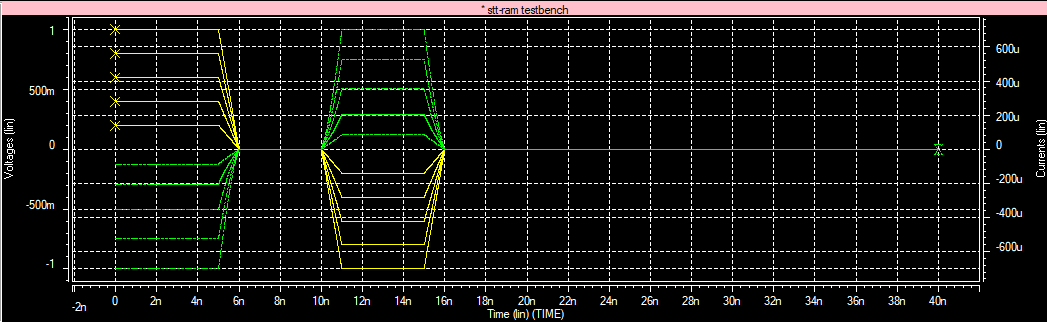
\includegraphics[width=1\textwidth]{images/img8}
%	\caption{خروجی شبیه‌سازی}
%	\label{خروجی شبیه‌سازی}
%\end{figure}

		
		
		
		
		
		
	\section*{سوالات شبیه‌سازی}
	\question
	
	
در این بخش از تکلیف خود، شما با شبیه‌ساز \lr{MNSIM 2.0} برای پیاده‌سازی یک شتاب‌دهنده شبکه عصبی سر و کار خواهید داشت. بنابراین، ابتدا باید این شبیه‌ساز را دانلود کرده و نتایج را طبق درخواست ارائه دهید.
	
	\subsection*{پیکربندی پایه:}
	\begin{enumerate}
		\item پارامتر‌های شبکه‌عصبی \lr{VGG8} که بر روی مجموعه داده \lr{CIFAR-10} آموزش دیده است را دانلود کنید، همانطور که در راهنمای \lr{MNSIM 2.0} توضیح داده شده است.
		\item برای هر اجرا، باید \lr{VGG8} را به عنوان شبکه عصبی مورد نظر خود انتخاب کنید.
	\end{enumerate}
	
	\textbf{پاسخ:} وزن ها را از \href{https://onedrive.live.com/?authkey=%21ANiQIk04073Gdfo&id=8F6F3FD340AC68D1%21332&cid=8F6F3FD340AC68D1}{\textcolor{magenta}{اینجا}}
	دانلود می‌کنیم.
	
	پس از دانلود به مسیر شبیه‌ساز می‌رویم و با دستور 
	
	\subsection*{سوال 1:}
	
	همانطور که در کلاس یاد گرفتید، ساختار \lr{PIM} شامل تعدادی کاشی است و هر کاشی شامل تعدادی \lr{PE} است. در هر \lr{PE}، ما مدارهای ضروری و ساختار ضربدری سلول‌های حافظه را داریم. اگر اندازه ضربدری را کاهش دهیم چه اتفاقی می‌افتد؟ به عنوان مثال، آیا باید انتظار داشته باشیم که توان، تأخیر و دقت کاهش، افزایش یا تغییر نکند؟ پاسخ خود را به تفصیل توضیح دهید.
	
	
	
	\textbf{پاسخ:}
کاهش اندازه‌ی ساختار کراسبار در معماری \lr{PIM} شامل چندین موازنه می‌شود و بر پارامترهای مختلفی مانند توان مصرفی، تأخیر و دقت تأثیر می‌گذارد. در ادامه به بررسی و تاثیر هر کدام می‌پردازیم:
	
	\section{توان مصرفی}
	\begin{itemize}
		\item \textbf{کاهش توان مصرفی:} کراسبارهای کوچکتر معمولاً به کاهش توان مصرفی منجر می‌شوند. این امر به این دلیل است که کراسبار کوچکتر تعداد سلول‌های حافظه و اتصالات کمتری دارد، که منجر به کاهش کلی ظرفیت خازنی می‌شود. ظرفیت کمتر به معنی شارژ/دشارژ کمتر در طول عملیات است که به توان مصرفی دینامیک کمتری منجر می‌شود.
		\item \textbf{ملاحظات توان استاتیک:} با این حال، توان مصرفی استاتیک ممکن است به همان اندازه کاهش نیابد، به ویژه اگر به همان تعداد مدارهای جانبی (مانند \lr{Sense amplifier} و درایورها) برای کراسبار کوچکتر نیاز باشد. کاهش در توان استاتیک عموماً کمتر از کاهش در توان دینامیک است.
	\end{itemize}
	
	\section{تأخیر}
	\begin{itemize}
		\item \textbf{کاهش تأخیر:} کراسبارهای کوچکتر می‌توانند تأخیر را بهبود بخشند. زمان خواندن یا نوشتن داده در یک ساختار کراسبار به طول اتصالات و تعداد سلول‌های حافظه وابسته است. با کراسبار کوچکتر، سیگنال‌ها باید مسافت کمتری را طی کنند و سلول‌های کمتری برای شارژ یا دشارژ وجود دارند، که منجر به عملیات سریعتر می‌شود.
	\end{itemize}
	
	\section{دقت}
	\begin{itemize}
		\item \textbf{بهبود بالقوه در دقت:} کراسبارهای کوچکتر می‌توانند منجر به بهبود دقت شوند. کراسبارهای بزرگتر با مشکلاتی مانند افزایش مقاومت و ظرفیت خازنی در طول اتصالات مواجه می‌شوند، که می‌تواند باعث تخریب سیگنال و افزایش حساسیت به نویز شود. با کاهش اندازه‌ی کراسبار، این اثرات به حداقل می‌رسند، که منجر به انتقال سیگنال و حسگری قابل اعتمادتر می‌شود و می‌تواند دقت را بهبود بخشد.
		\item \textbf{نرخ خطا:} احتمال خطا به دلیل تداخل و سایر اثرات نیز در کراسبارهای کوچکتر کمتر است، که به بهبود دقت در عملیات‌هایی مانند ضرب ماتریسی و عملیات‌های برداری که به طور معمول در معماری \lr{PIM} استفاده می‌شوند، کمک می‌کند.
	\end{itemize}
	
	
	
	
	
	
	
	
	
	
	
	
	
	\subsection*{سوال 2:}
	
	اگر بخواهیم \lr{PUM} را به این شبیه‌ساز اضافه کنیم، کدام قسمت باید تغییر کند؟
	
	
\textbf{پاسخ:‌ }

تغییرات مورد نیاز برای اضاف کردن \lr{PUM} به شبیه‌ساز \lr{NVSim} به‌صورت زیر است:

\subsection*{قسمت‌های کلیدی برای تغییر}

\begin{enumerate}
	\item \textbf{پیکربندی سخت‌افزار (\lr{\texttt{SimConfig.ini}}):}
	\begin{itemize}
		\item می‌بایست معماری \lr{PUM} را در فایل پیکربندی سخت‌افزار توصیف کنیم.
		
		\item بر اساس معماری مورد نیاز خودمان می‌توانیم بخش‌هایی را به فایل کانفیگ اضافه نموده. این بخش‌ها شامل اضاف نمودن پارامتر‌های سخت افزاری \lr{PUM} مانند نوع حافظه، الگو‌های دسترسی حافظه و ... باشد
	\end{itemize}
	
	
	
	
برای مثال می‌توان این تنظیمات را در فایل \texttt{SimConfig.ini} انجام داد:
	\begin{latin}
		\begin{verbatim}
			[PUM]
			um_enabled = True
			memory_type = "RRAM"
			access_pattern = "row-major"
			pum_specific_param1 = value1
			pum_specific_param2 = value2
		\end{verbatim} 
	\end{latin}
	
	
	\begin{figure}[h]
		\centering
		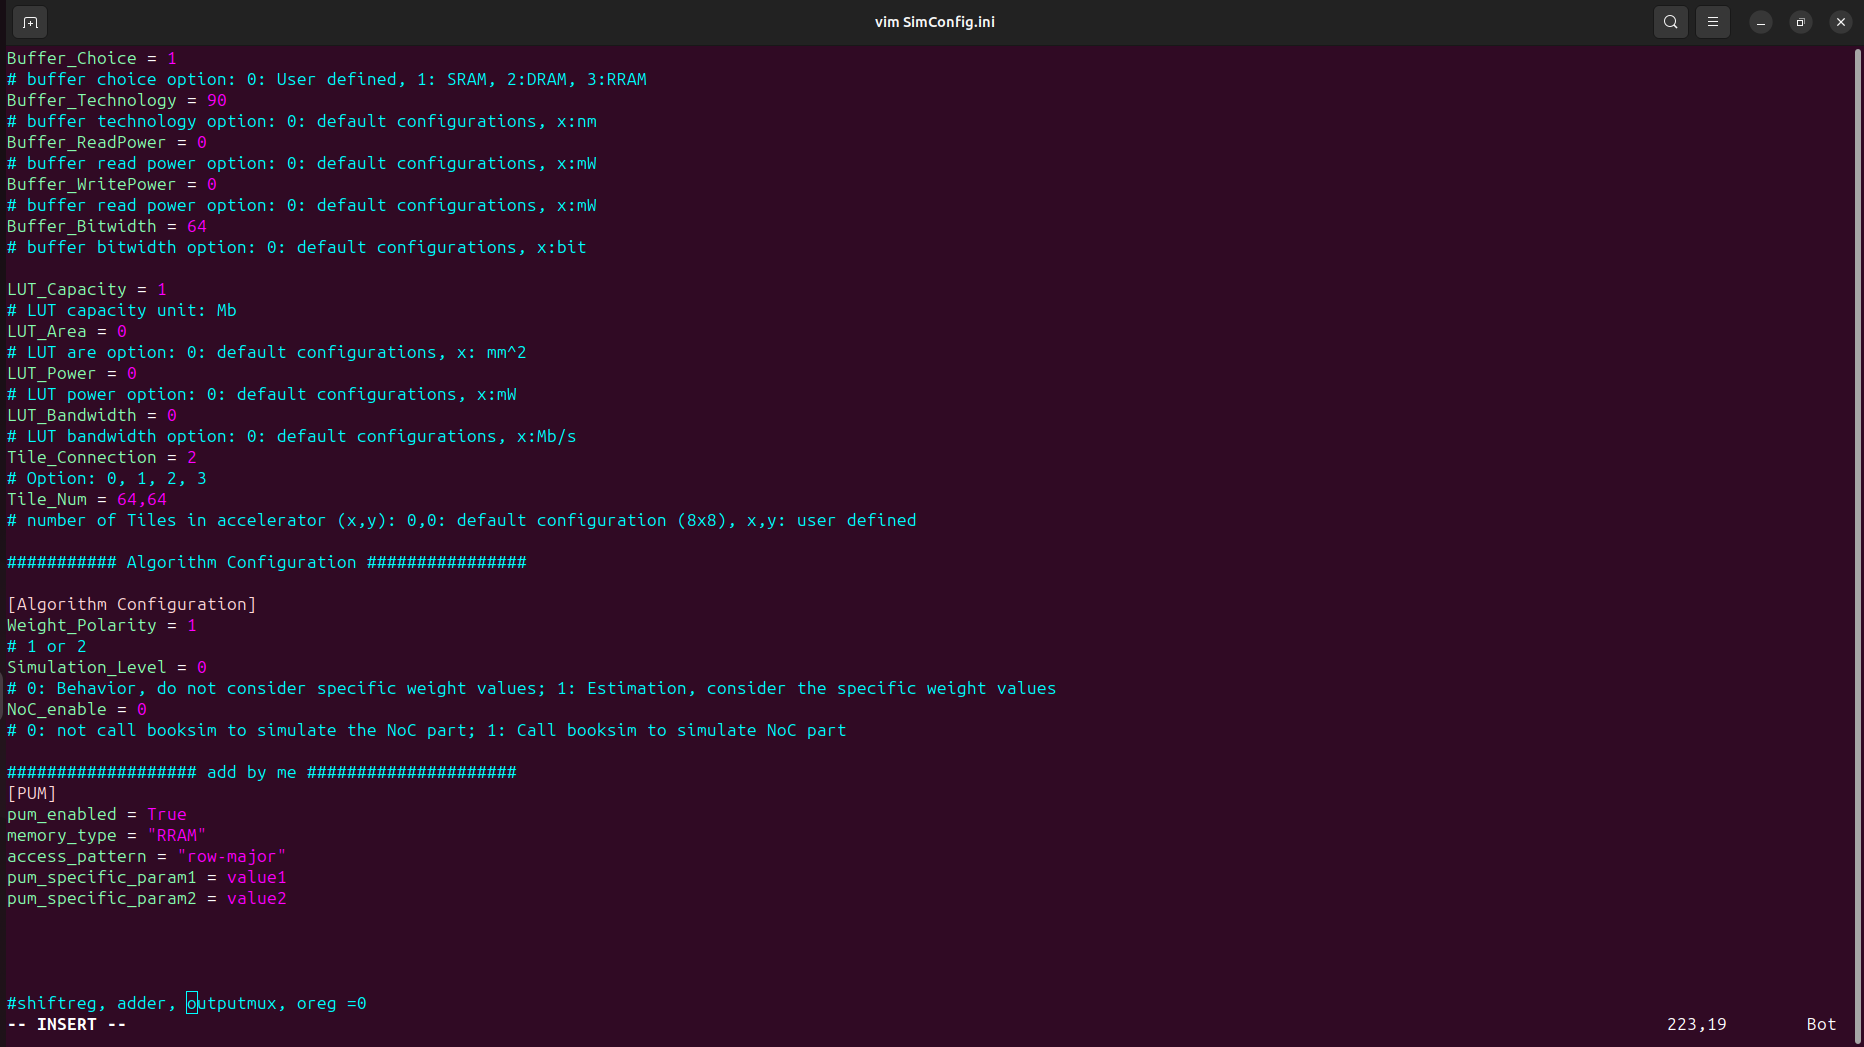
\includegraphics[width=1\textwidth]{images/6-Add_PUM_to_SimConfig.png}
		\caption{اضافه کردن کانفیگ \lr{PUM}}
		\label{اضافه کردن کانفیگ PUM}
	\end{figure}
	
	
	
	

	
	
	\item \textbf{توصیف شبکه (\lr{\texttt{network.py}}):}
	
	اگر فایل \texttt{network.py} را باز کنیم، مشاهده می‌کنیم که همه تنظیمات لایه‌های مختلف شبکه در این فایل تنظیم شده است. می‌بایست این فایل را طوری تغییر دهیم که معماری \lr{PUM} را به لایه‌های مختلف اضافه کنیم و آن را با لایه‌های مختلف ارتباط دهیم. برای انجام تغییرات باید به مسیر زیر برویم:
	\begin{latin}
		\begin{verbatim}
			MNSIM/Interface/
		\end{verbatim} 
	\end{latin}
	
	برای مثال می‌توان مطابق با سایر تنظیمات همین فایل، یک \texttt{if} دیگر به کد ها اضافه کرد.
	
	\begin{latin}
		\begin{verbatim}
			if(cate.startswith('pum_net')):
				    layer_config_list.append({'type': 'pum_conv', 'in_channels': 3,
					     'out_channels': 64, 'kernel_size': 3, 'padding': 1, 'stride': 2})
				    layer_config_list.append({'type': 'relu'})
				    layer_config_list.append({'type': 'pooling', 'mode': 'MAX',
				       'kernel_size': 2, 'stride': 2})
		\end{verbatim} 
	\end{latin}
	
	\begin{figure}[h]
		\centering
		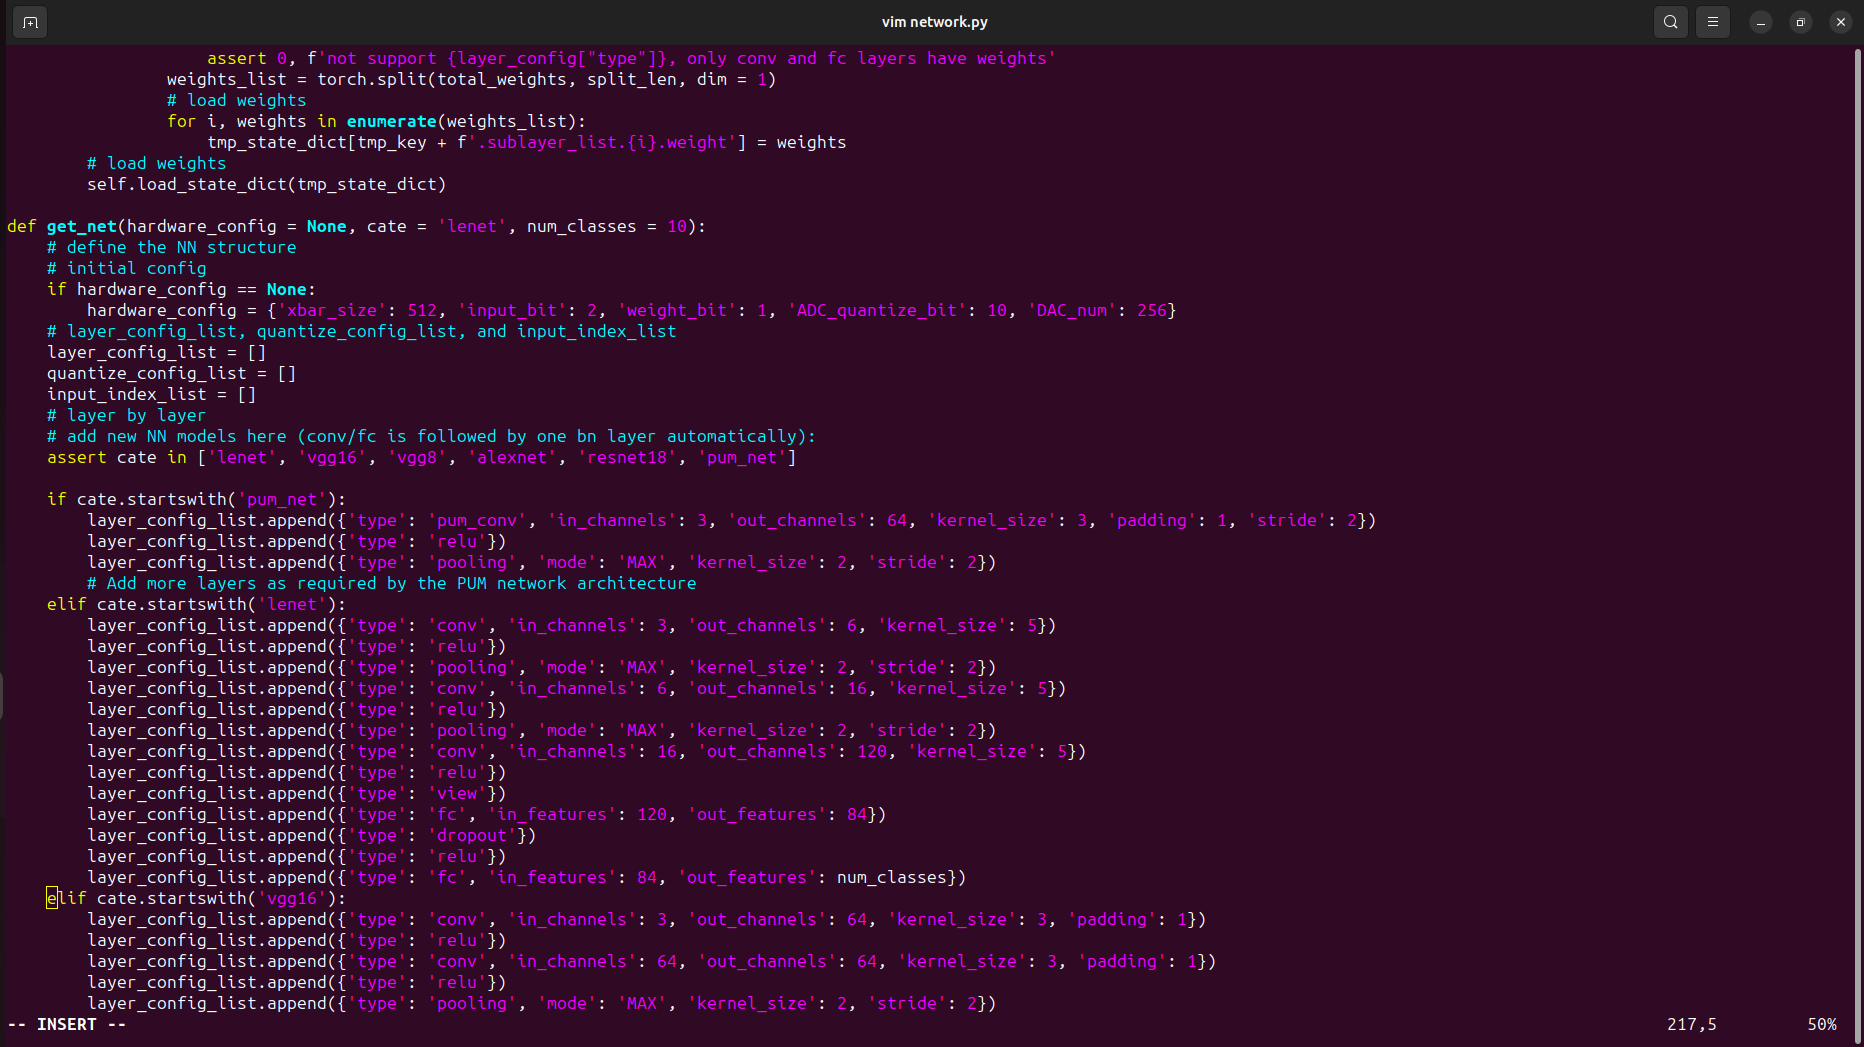
\includegraphics[width=1\textwidth]{images/7-Add_PUM_to_network.png}
		\caption{اضافه کردن \lr{PUM} به فایل \texttt{network.py}}
		\label{اضافه کردن PUM به فایل network}
	\end{figure}
	
	
	\item \textbf{تغییر ماژول‌های شبیه‌سازی:}\\
	
	پس از مرتبط کردن لایه‌های شبکه با معماری \lr{PUM} مورد نظر، می‌بایست توابع پیاده سازی آن نیز در سایر فایل‌های برنامه تعریف شود. برای انجام این کار می‌بایست به مسیر زیر برویم:
	
	\begin{latin}
		\begin{verbatim}
			MNSIM/Hardware_Model/ 
		\end{verbatim} 
	\end{latin}
	
	و فایل های زیر را مطابق با نیاز‌هایمان تغییر دهیم:
	\begin{latin}
		\begin{enumerate}
			\item \texttt{Crossbar.py}
			\item \texttt{PE.py}
			\item \texttt{Device.py}
			\item \texttt{Crossbar.py}
			\item \texttt{PE.py}
			\item \texttt{Tile.py}
			\item \texttt{Buffer.py}
		\end{enumerate} 
	\end{latin}
\end{enumerate}
	
	
	
	
	
	
\subsection*{سوال 3:}
	
در اولین پیاده‌سازی، ابعاد ضربدری (\lr{Xbar}) را به \lr{256x256} تنظیم کنید. در پیاده‌سازی دوم، ابعاد ضربدری را به \lr{128x128} تغییر دهید. مجموع تأخیر، توان و انرژی را گزارش دهید و جدول را پر کنید. چه اتفاقی افتاد؟ چرا؟ (برای هر پارامتر به تفصیل توضیح دهید.)


\textbf{پاسخ: }

به‌صورت پیش‌فرض \lr{Xbar} سایز بر روی \lr{256x256} تنظیم است. پس از نصب کتابخانه‌های مورد نیاز مثل:


\begin{latin}
	\begin{enumerate}
		\item \texttt{numpy}
		\item \texttt{torch}
		\item \texttt{torch vision}
	\end{enumerate}
\end{latin}

در دایرکتوری شبیه‌ساز دستور زیر را اجرا می‌کنیم:

\begin{latin}
	\texttt{\textcolor{blue}{\$} python3 main.py}
\end{latin}

فرایند اجرا چند دقیقه‌ای به طول خواهد انجامید و سیستم به شدت داغ خواهد شد! پس از اتمام شبیه‌سازی خروجی به صورت شکل «\textcolor{blue}{\ref*{خروجی شبیه‌سازی با سایز256x256}}» زیر می‌شود:

\begin{figure}[h]
	\centering
	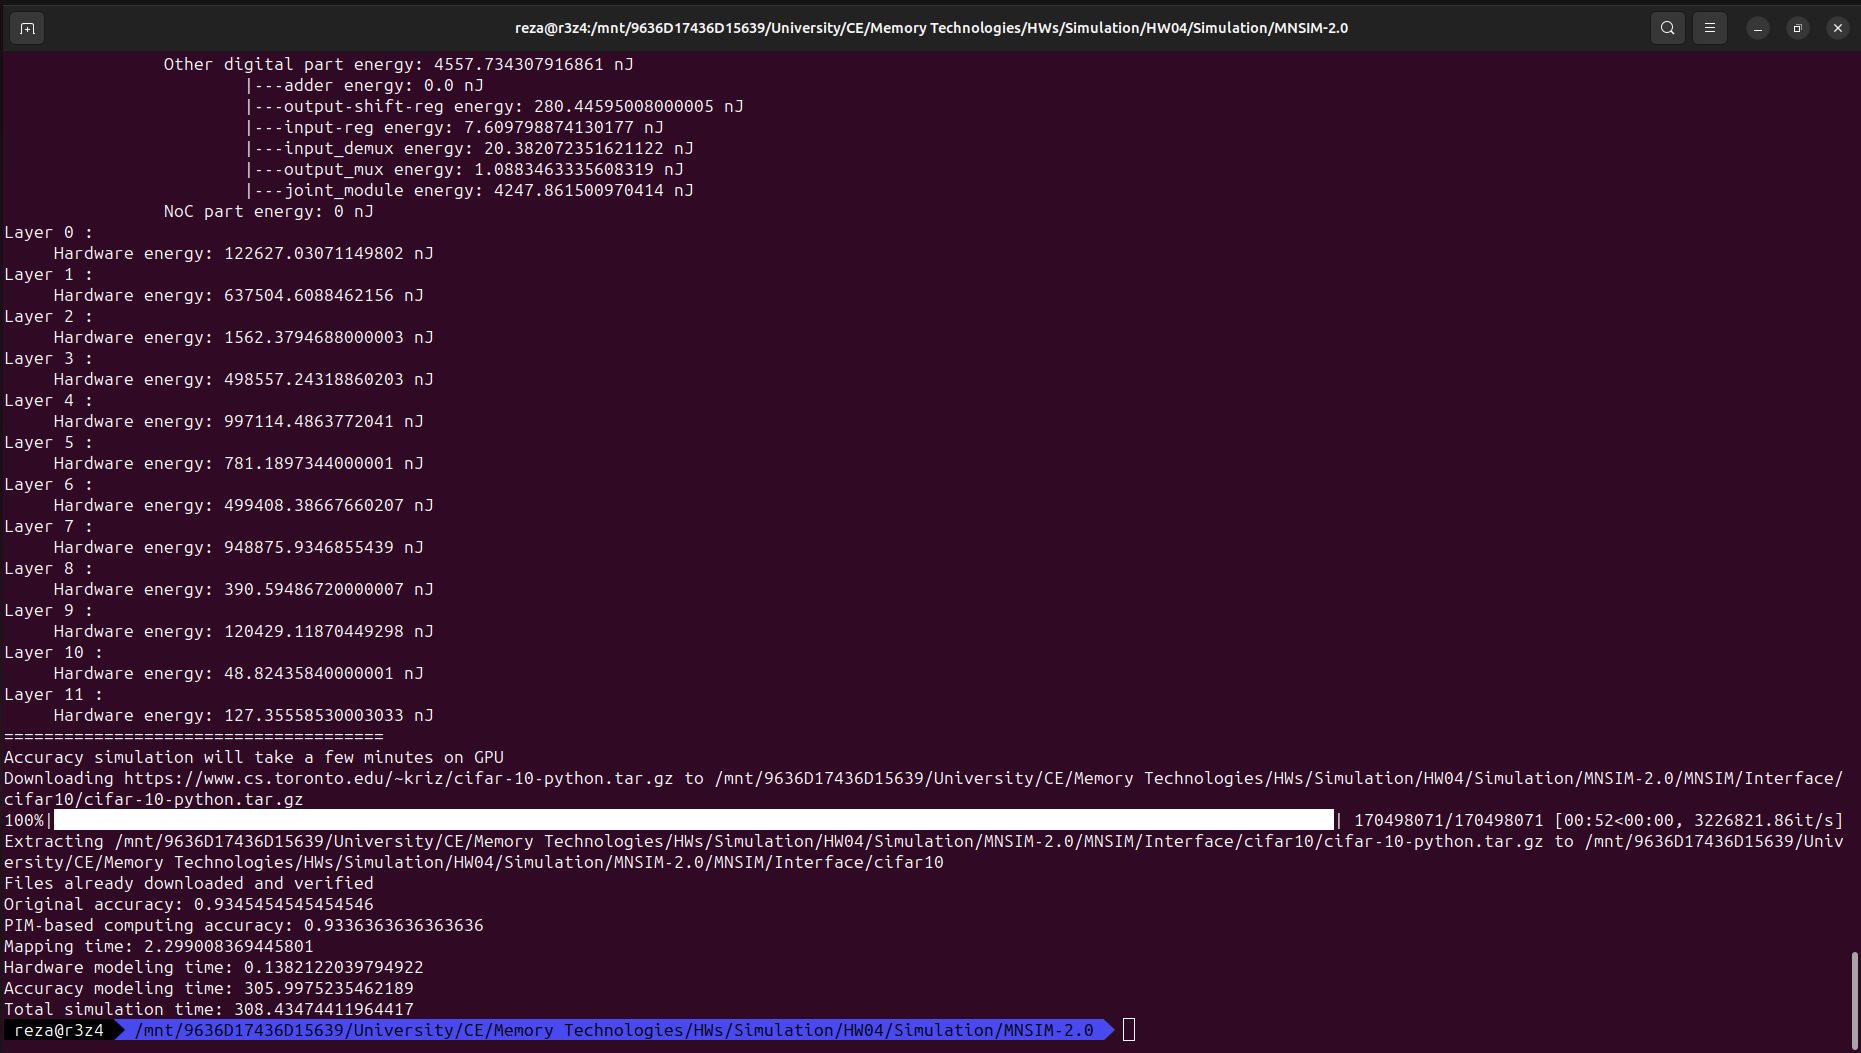
\includegraphics[width=1\textwidth]{images/256x256/0-main-py.png}
	\caption{خروجی شبیه‌سازی با سایز \lr{256x256}}
	\label{خروجی شبیه‌سازی با سایز256x256}
\end{figure}

اسکرین‌شات های خروجی همگی در مسیر \texttt{images/} قرار دارد.

در گام دوم از فایل \texttt{SimConfig.ini} مقدار \texttt{Xbar\_Size} را به \texttt{128,128} تغییر می‌دهیم و مجددا فایل را شبیه‌سازی می‌کنیم. خروجی شبیه‌سازی در شکل «\textcolor{blue}{\ref{خروجی شبیه‌سازی با 128x128}}»


\begin{figure}[h]
	\centering
	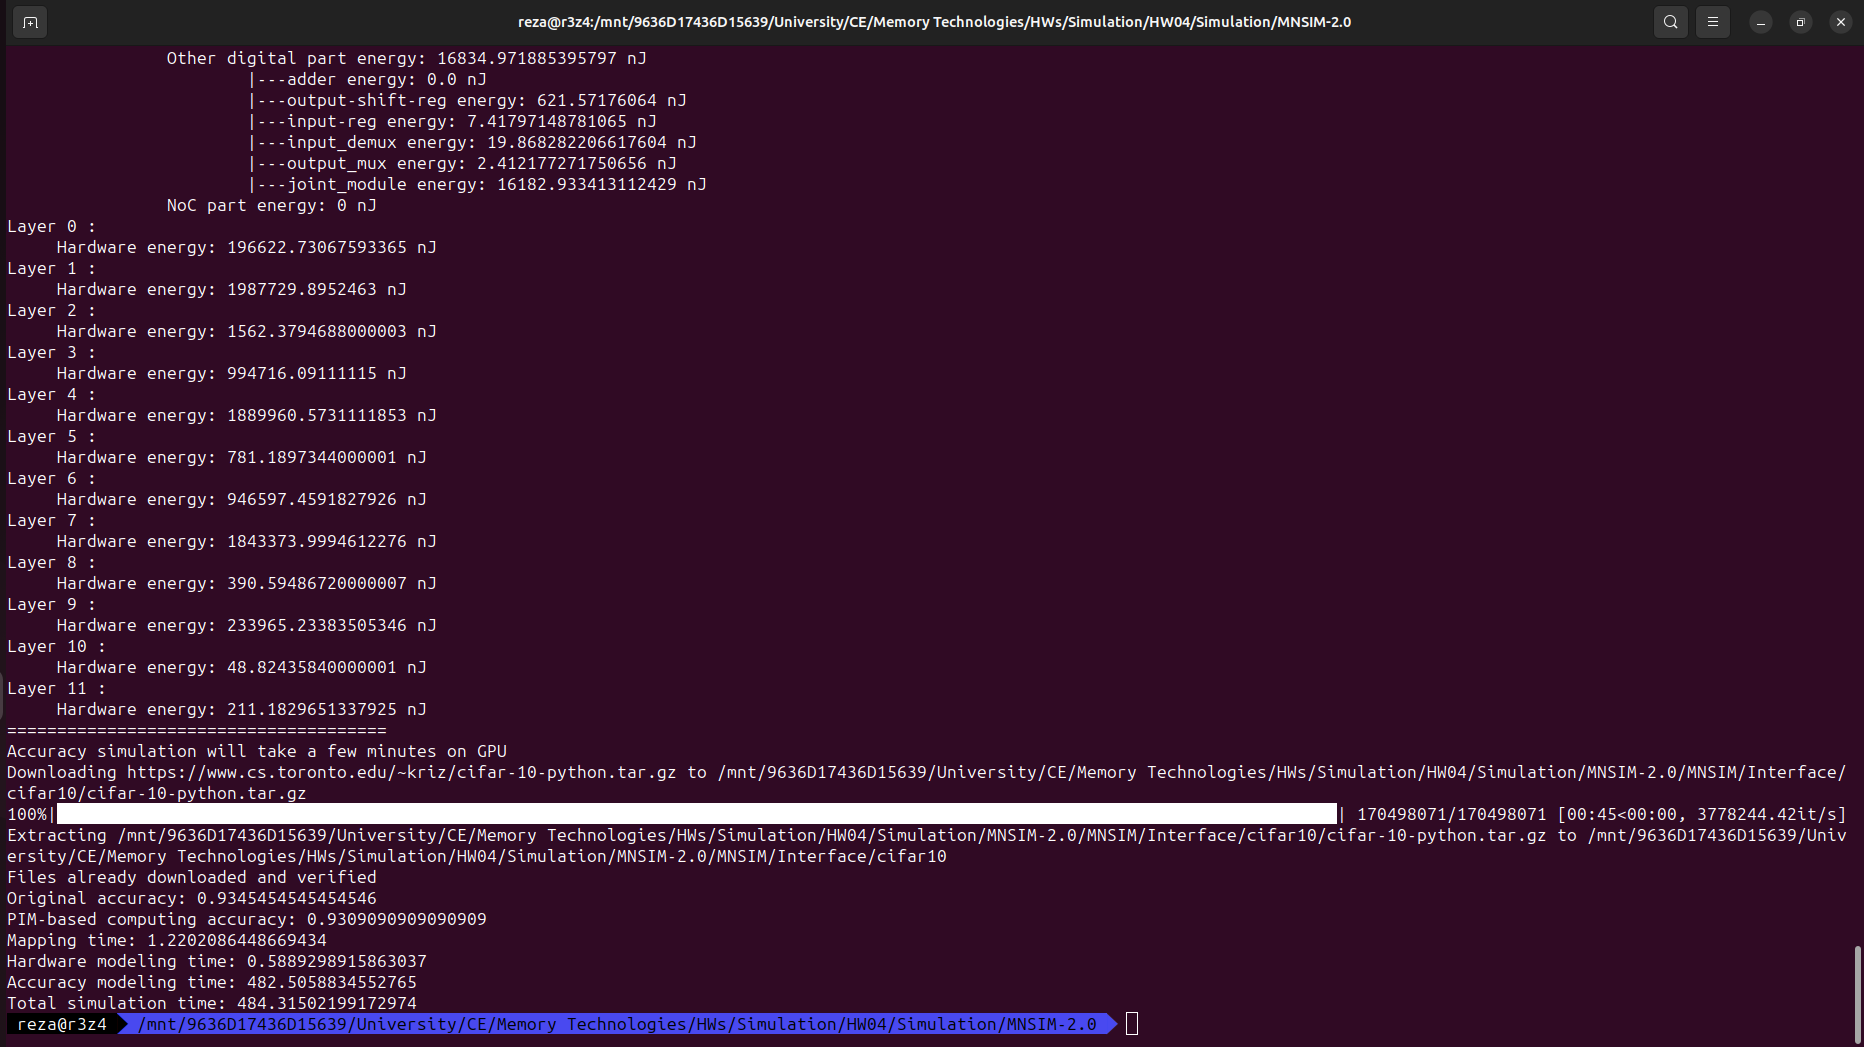
\includegraphics[width=1\textwidth]{images/128x128/0.png}
	\caption{خروجی شبیه‌سازی با سایز \lr{128x128}}
	\label{خروجی شبیه‌سازی با 128x128}
\end{figure}

با توجه به مقادیر به‌دست آمده از شبیه‌سازی، جدول «\textcolor{blue}{\ref*{جدول نتایج}}» را تکمیل می‌کنیم
	
	\begin{table}[h]
		\centering
		\begin{tabular}{|c|c|c|c|}
			\hline
			& \textbf{\lr{128*128}} & \textbf{\lr{256*256}} & \textbf{وضعیت} \\ \hline
			\textbf{تأخیر} & \lr{5288665.312627485 ns} & \lr{5330703.614503523 ns} & کاهش \\ \hline
			\textbf{توان} & \lr{1297.5432541884213 W} & \lr{338.62446474552047 W} & افزایش \\ \hline
			\textbf{انرژی} & \lr{8095960.154017576 nJ} & \lr{3827427.1532042585 nJ} & افزایش \\ \hline
		\end{tabular}
		\caption{نتایج شبیه‌سازی}
		\label{جدول نتایج}
	\end{table}
	
	\subsection*{توضیحات:}
	
	\begin{itemize}
		\item \textbf{تأخیر:} 
		کاهش ابعاد کراسبار از \lr{256x256} به \lr{128x128} باعث کاهش تأخیر شده است. این کاهش تأخیر به این دلیل است که کراسبار کوچک‌تر دارای مسیرهای انتقال داده کوتاه‌تر و پیچیدگی کمتری است، که منجر به کاهش زمان دسترسی و اجرای عملیات می‌شود. در نتیجه، مقدار تأخیر در کراسبار \lr{128x128 }کمتر از کراسبار \lr{256x256} است.
		
		\item \textbf{توان:}
		افزایش توان در کراسبار \lr{128x128} نسبت به \lr{256x256} به این دلیل است که با کاهش ابعاد کراسبار، تعداد عملیات‌های پردازشی و تعداد دفعات دسترسی به حافظه افزایش می‌یابد. این افزایش عملیات‌های پردازشی باعث افزایش مصرف توان داینامیک می‌شود. بنابراین، توان مصرفی در کراسبار \lr{128x128} بیشتر از کراسبار \lr{256x256} است.
		
		\item \textbf{انرژی:}
		افزایش انرژی مصرفی در کراسبار \lr{128x128} نسبت به \lr{256x256} نتیجه مستقیم افزایش توان مصرفی و تأثیر کمتر کاهش تأخیر است. اگرچه تأخیر کاهش یافته است، اما افزایش توان مصرفی بیشتر بوده و در نتیجه انرژی مصرفی نیز افزایش یافته است. انرژی مصرفی تابعی از توان و تأخیر است و افزایش توان به طور کلی تأثیر بیشتری بر افزایش انرژی دارد. بنابراین، انرژی مصرفی در کراسبار \lr{128x128} بیشتر از کراسبار \lr{256x256} است.
	\end{itemize}
	
	
	
	\section*{سوال 4:}
	در برخی لایه‌ها، توان ثابت است در حالی که تأخیر متفاوت است. علت چیست؟
	
	\textbf{پاسخ:‌ }
	
	\begin{enumerate}
		\item \textbf{نوع عملیات در لایه‌ها:}
		لایه‌های مختلف شبکه عصبی (مانند لایه‌های کانولوشن، لایه‌های \lr{Fully connected} و توابع فعال‌ساز) ممکن است عملیات‌های مختلفی را انجام دهند که نیاز به محاسبات و زمان متفاوتی دارند. حتی اگر توان مصرفی ثابت باشد، نوع و پیچیدگی عملیات می‌تواند باعث تغییر در تأخیر شود. به عنوان مثال، لایه‌های کانولوشن معمولاً به عملیات محاسباتی پیچیده‌تری نسبت به توابع فعالسازی نیاز دارند که می‌تواند تأخیر بیشتری ایجاد کند.
		
		\item \textbf{تعداد عملیات‌های موازی:}
		تعداد عملیات‌هایی که به صورت موازی در یک لایه اجرا می‌شوند می‌تواند تأثیر زیادی بر تأخیر داشته باشد. در لایه‌هایی که موازی‌سازی بیشتری دارند، تأخیر می‌تواند کاهش یابد حتی اگر توان مصرفی ثابت بماند. این موازی‌سازی می‌تواند وابسته به اندازه کراسبار و نحوه تقسیم وظایف بین واحدهای پردازشی باشد.
		
		\item \textbf{بار حافظه و دسترسی به داده‌ها:}
		نحوه دسترسی به داده‌ها و بار حافظه می‌تواند باعث تفاوت در تأخیر شود. حتی اگر توان مصرفی ثابت باشد، تأخیر دسترسی به حافظه و انتقال داده‌ها می‌تواند متفاوت باشد. لایه‌هایی که به داده‌های بیشتری نیاز دارند یا دسترسی‌های بیشتری به حافظه دارند، ممکن است تأخیر بیشتری داشته باشند.
		
		\item \textbf{تفاوت در الگوهای دسترسی به حافظه:}
		الگوهای دسترسی به حافظه در لایه‌های مختلف می‌تواند متفاوت باشد. به عنوان مثال، لایه‌هایی که نیاز به دسترسی تصادفی بیشتری دارند، ممکن است تأخیر بیشتری را تجربه کنند در حالی که توان مصرفی ثابت باقی می‌ماند. این تفاوت در الگوهای دسترسی می‌تواند به علت ساختار داده‌ها و نیازهای محاسباتی خاص هر لایه باشد.
	\end{enumerate}
	
	
	
	
	\section*{سوال 5:}
	کدام اندازه کراسبار بهتر است؟ لطفاً با جزئیات توضیح دهید. برای مثال، اگر تصمیم شما بر اساس توان، تأخیر یا انرژی است، باید علت و دلیل این شرایط را ذکر کنید.
	
	
	
با توجه به نتایج بدست آمده از شبیه‌سازی (جدول «\textcolor{blue}{\ref*{جدول نتایج}}») می‌توان گفت:

\begin{enumerate}
	\item
	کراسبار \lr{128x128} تأخیر کمتری نسبت به کراسبار \lr{256x256} دارد. کاهش تأخیر به معنای سریع‌تر انجام شدن عملیات‌ها و پردازش‌هاست که می‌تواند در برنامه‌هایی که نیاز به سرعت بالا دارند، مزیت بزرگی باشد.
	
	\item
	کراسبار \lr{128x128} توان بیشتری نسبت به کراسبار \lr{256x256} مصرف می‌کند. افزایش توان مصرفی به معنای نیاز به منابع انرژی بیشتر و احتمال افزایش گرما در سیستم است که می‌تواند به مشکلات حرارتی و نیاز به خنک‌سازی منجر شود.
	
	\item
	انرژی مصرفی در کراسبار \lr{128x128} بیشتر از کراسبار \lr{256x256} است. انرژی مصرفی تابعی از توان و تأخیر است و افزایش انرژی به معنای کارایی کمتر از نظر مصرف انرژی است.
\end{enumerate}



	بنابر این با توجه به معیار ما برای انتخاب می‌توان یکی از حالت‌های زیر را انتخاب کرد:
	\begin{itemize}
		\item \textbf{اگر اولویت تاخیر باشد:}
		کراسبار \lr{128x128} گزینه بهتری است زیرا تأخیر کمتری دارد و عملیات‌ها را سریع‌تر انجام می‌دهد.
		
		\item \textbf{اگر اولویت توان و انرژی مصرفی باشد:}
		کراسبار \lr{256x256} گزینه بهتری است زیرا توان و انرژی کمتری مصرف می‌کند که می‌تواند به کاهش هزینه‌ها و مشکلات حرارتی کمک کند.
	\end{itemize}
	
	
 \end{questions}

\end{document}